\documentclass{beamer}
\usepackage[english]{babel}
\usepackage[utf8]{inputenc}
\usepackage{multicol}
\usepackage{graphicx}
\usepackage{subfig}
\usepackage{hyperref}
\hypersetup{
    colorlinks=true,
    linkcolor=blue,
    filecolor=magenta,      
    urlcolor=blue,
}
%\usepackage[shortlabels]{enumitem}
\usepackage{amsmath,amsthm, amssymb, latexsym}

\usetheme{Frankfurt}
\usefonttheme[onlymath]{serif}
\setbeamertemplate{caption}[numbered]
\setbeamertemplate{enumerate items}[default]
\setbeamertemplate{bibliography item}{\insertbiblabel}
\usepackage[orientation=landscape, size=a0]{beamerposter}

\usepackage[absolute, overlay]{textpos}
\setlength{\TPHorizModule}{\paperwidth}
\setlength{\TPVertModule}{\paperheight}

\title{\huge Boundary Effects in Stochastic Cyclic Competition Models on a Two-Dimensional Lattice}
\author{\Large M. Lazarus Arnau, Shannon Serrao, Uwe C. T{\"a}uber}
\institute{\normalsize Department of Physics (MC 0435) and Center for Soft Matter and Biological Physics\\ Virginia Tech, Blacksburg, Virginia 24061}
\date{October 13, 2018}

\begin{document}
\begin{frame}{}

%Left Col
\begin{textblock}{0.32}(0.01,0.015)
    \begin{block}{\centering Introduction}
        \begin{figure}[h]
            \centering
            \subfloat[]{{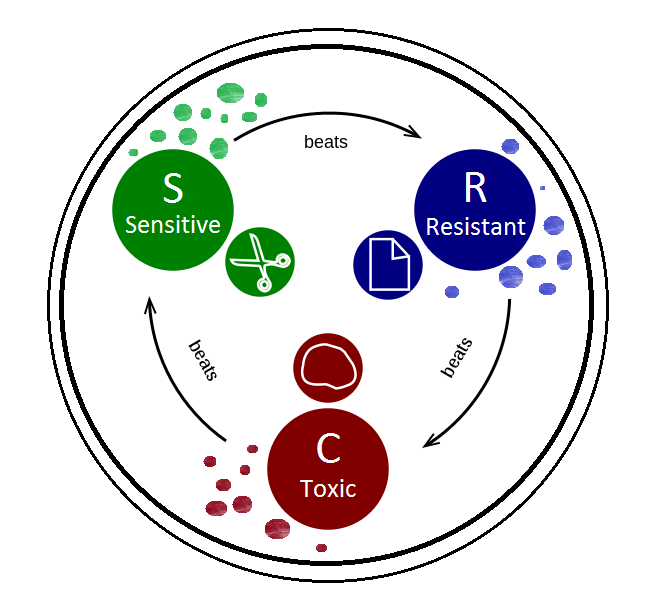
\includegraphics[width=0.4\linewidth]{images/ecolirps.png} }}
            \subfloat[]{{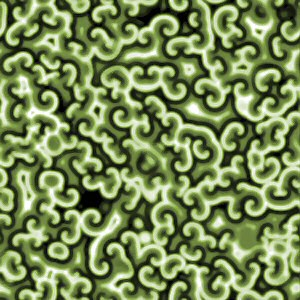
\includegraphics[width=0.4\linewidth]{images/Belousov-Zhabotinsky.jpg} }}
            \caption{(a) Cyclic dominance in \textit{E. coli} (b) Spiral pattern formation in the Belousov-Zhabotinsky reaction.}
            \label{fig:images}
        \end{figure}
        A number of systems in the fields of ecology, epidemiology, and chemistry
        follow a paradigm of cyclic dominance or have been shown to exhibit noise-induced 
        pattern formation (e.g. certain subspecies of Lizards in
        California \cite{sinervo96}, experiments on cyclically competing \textit{E. coli} bacteria \cite{kerr02}, and
        the Belousov-Zhabotinsky reaction \cite{epstein96}). The formation of noise-induced and -stabilized
        spiral patterns in this class of system is captured by the spatially-extended 
        May-Leonard (ML) model. The formation of these spirals is in stark contrast
        to the species clustering seen in the Rock-Paper-Scissors (RPS) model.        
    \end{block}
    \begin{block}{\centering The RPS Model}
        The RPS Model is defined by the following binary reactions:
        \begin{itemize}
            \item Replacement reaction:
            \begin{gather*}
                AB \rightarrow AA\\
                BC \rightarrow BB\\
                CA \rightarrow CC\\            
                \text{with rate } \zeta
            \end{gather*}

            \item Pair swap / diffusion reaction:
            \begin{gather*}
                XY \rightarrow YX \\
                \text{where }X, Y \in \{A, B, C, \varnothing\} \text{ with rate } \epsilon_r
            \end{gather*}
        \end{itemize}
    \end{block}
    \begin{block}{\centering The May-Leonard Model}
        The ML Model is defined by the following binary reactions:
        \begin{itemize}
            \item Predation reaction:
            \begin{gather*}
                AB \rightarrow A \varnothing \\
                BC \rightarrow B \varnothing \\
                CA \rightarrow C \varnothing \\            
                \text{with rate } \sigma
            \end{gather*}
            \item Reproduction reaction:
            \begin{gather*}
                A \varnothing \rightarrow AA\\
                B \varnothing \rightarrow BB\\
                C \varnothing \rightarrow CC\\            
                \text{with rate } \mu
            \end{gather*}
            \item Pair swap / diffusion reaction:
            \begin{gather*}
                XY \rightarrow YX \\
                X, Y \in \{A, B, C, \varnothing\} \text{ with rate } \epsilon_m
            \end{gather*}
        \end{itemize}

    \end{block}
    \begin{block}{\centering Simulation}
        We define $x$ to be the vertical (short) axis and $y$ to be the horizontal
        (long) axis. A lattice of size $L_x \times L_y$ is then initialized with each cell 
        being assigned a random species with probability $p (A) = p (B) = p (C) = {\rho_0}/{3}$ (where $\rho_0$ is the 
        initial net particle density). We limit each lattice point to contain at most
        one particle.
        The lattice is given a toroidal topology (i.e. $x=0 \text{ is equivalent 
        to } x = L_x$ and likewise for $y = L_y$). The simulation then proceeds according 
        to the following algorithm:

        \begin{enumerate}
            \item A random coordinate $(x, y)$ is selected from a uniform distribution
                and time is advanced by $\delta t = N^{-1} $ (where $N = L_x \times L_y$).
            \item If that lattice point is not empty, then a nearest neighbor is chosen
                at random. If the cell is empty, the simulation returns to step 1.
            \item One of the possible reactions (as determined by the model) is 
                selected at random (with probability determined by the reaction 
                rates), and excecuted if possible. The simulation returns to step 1.
        \end{enumerate}

        In cases where there are both RPS and ML lattice points, all lattice points
        in the range $0 \leq y < d_i$ are governed by the RPS model and all 
        remaining lattice points are governed by the ML model.
    \end{block}
\end{textblock}

%Middle Collumn
\begin{textblock}{0.32}(0.34, 0.0125)
    \begin{block}{}
        \maketitle
        \centering
        We study noise-induced and -stabilized spatial patterns in two distinct stochastic 
        population model variants for cyclic competition of three species, namely the 
        Rock-Paper-Scissors (RPS) and the May-Leonard (ML) models. In two dimensions, 
        it is well established that the ML model can display (quasi-)stable spiral 
        structures, in contrast to simple species clustering in the RPS system. Our 
        ultimate goal is to impose control over such competing structures in systems 
        where both RPS and ML reactions are implemented. To this end, we have employed 
        Monte Carlo computer simulations to investigate how changing the microscopic 
        rules in a subsection of a two-dimensional lattice influences the macroscopic 
        behavior in the rest of the lattice. Specifically, we implement the ML reaction scheme 
        on a torus, except on a ring-shaped patch, which is set to follow the cyclic 
        Lotka-Volterra predation rules of the RPS model. There, we observe a marked disruption of 
        the usual spiral patterns in the form of plane waves emanating from the RPS region.
        Furthermore, the overall population density drops considerably in the 
        vicinity of the interface between both regions. 
    \end{block}
    \begin{block}{\centering Normal Pattern Formation}
        \begin{figure}[h]
            \centering
            \subfloat[$\epsilon_m=0.1$]{{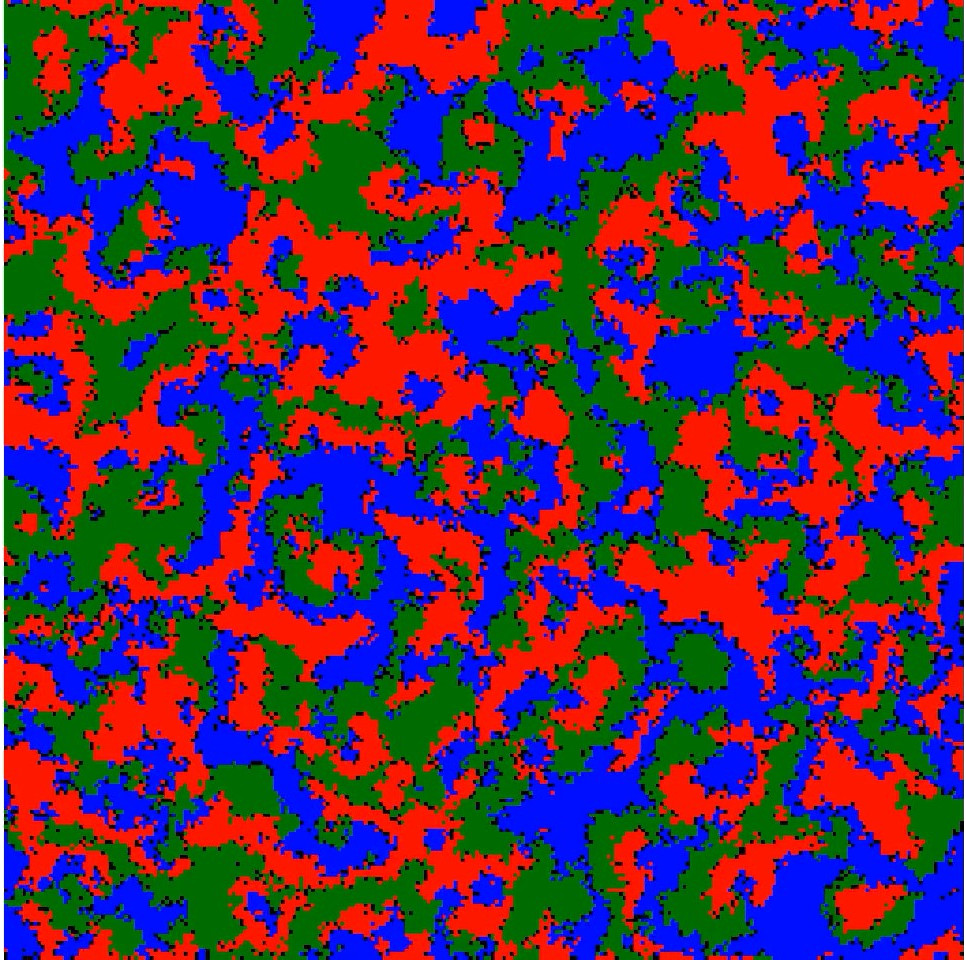
\includegraphics[width=0.24\linewidth]{images/ml_0_1.jpg} }}
            \subfloat[$\epsilon_m=1.25$]{{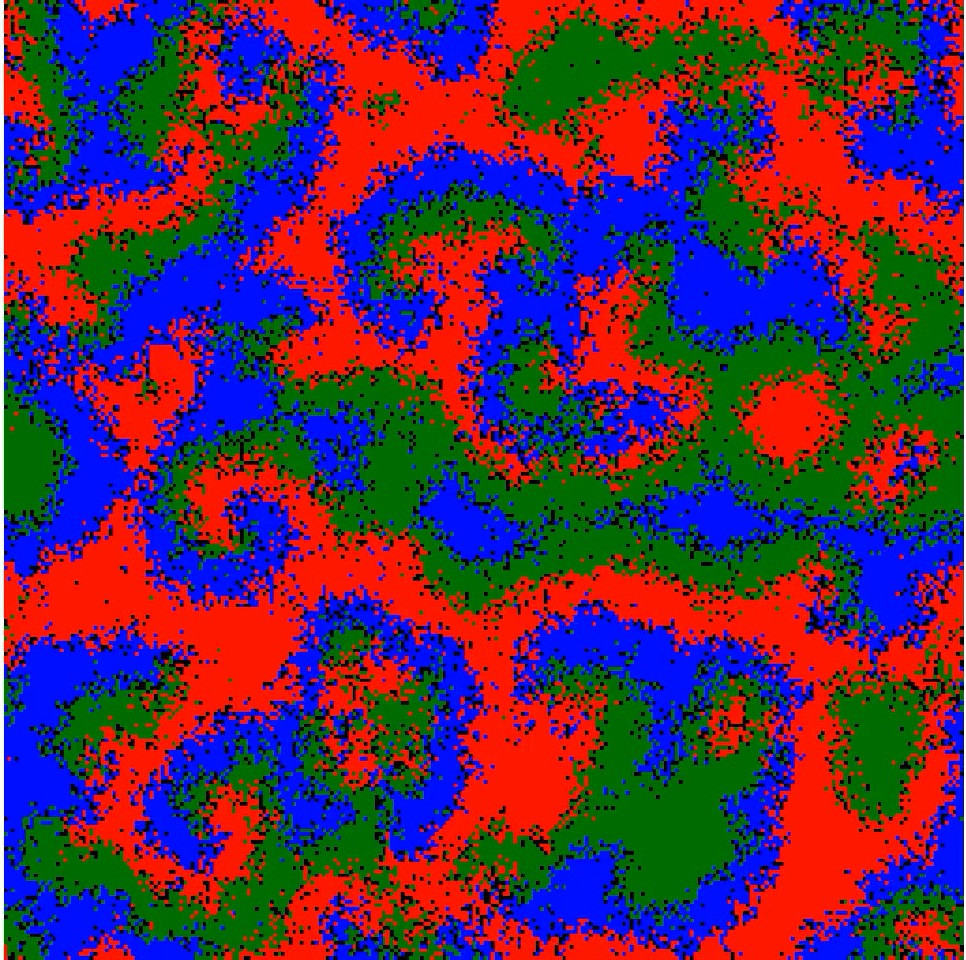
\includegraphics[width=0.24\linewidth]{images/ml_1_25.jpg} }}
            \subfloat[$\epsilon_m=5.0$]{{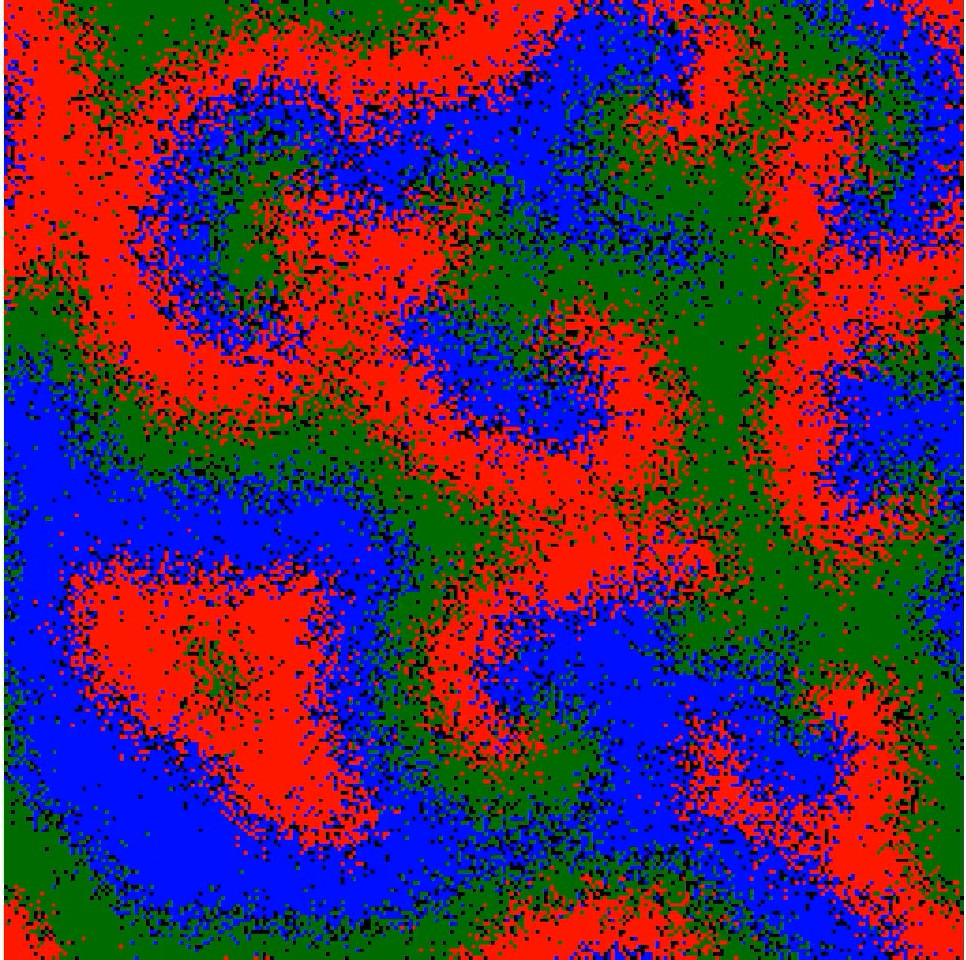
\includegraphics[width=0.24\linewidth]{images/ml_5_0.jpg} }}
            \subfloat[$\epsilon_m=10.0$]{{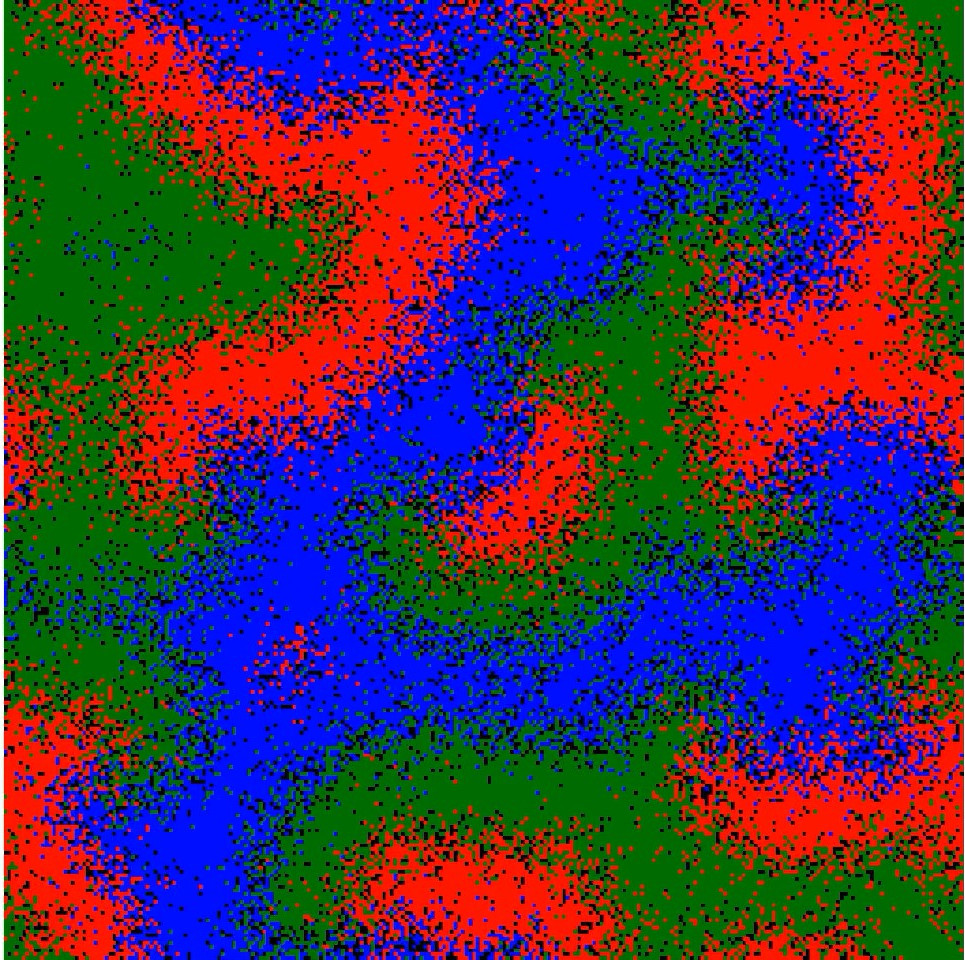
\includegraphics[width=0.24\linewidth]{images/ml_10_0.jpg} }}
            \\
            \subfloat[$\epsilon_r=0.1$]{{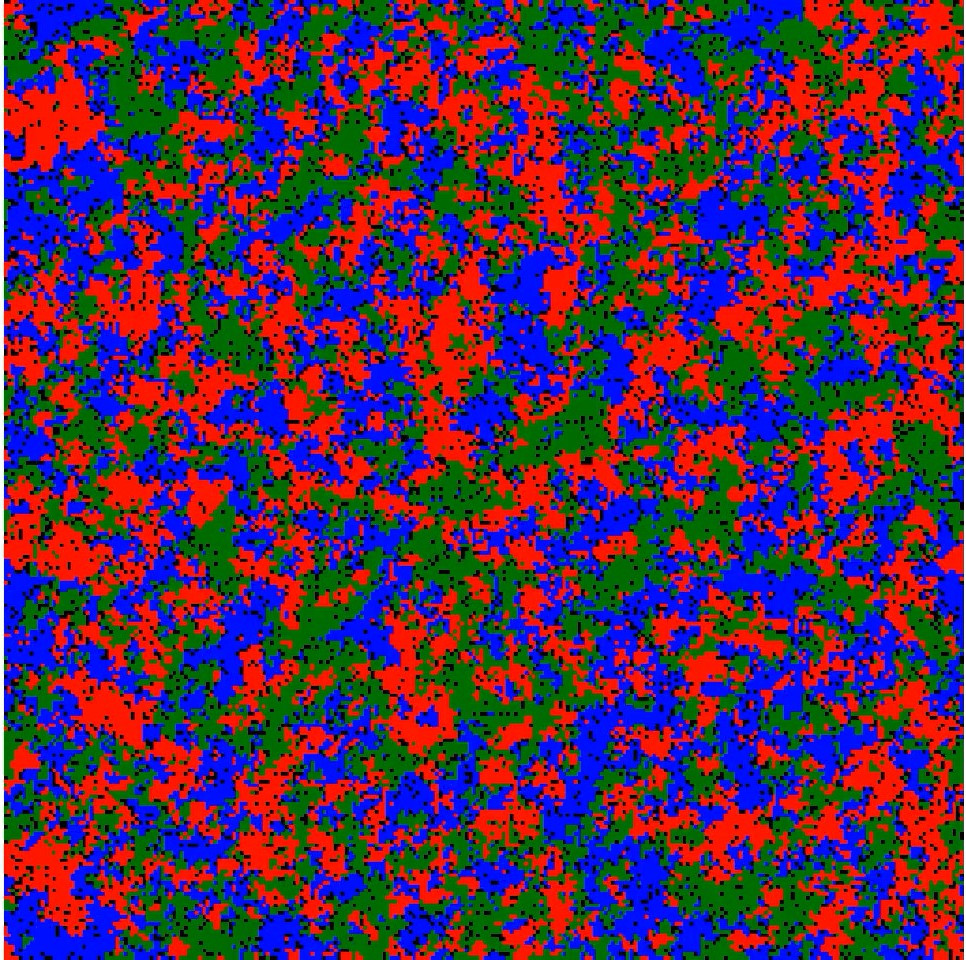
\includegraphics[width=0.24\linewidth]{images/rps_0_1.jpg} }}
            \subfloat[$\epsilon_r=1.25$]{{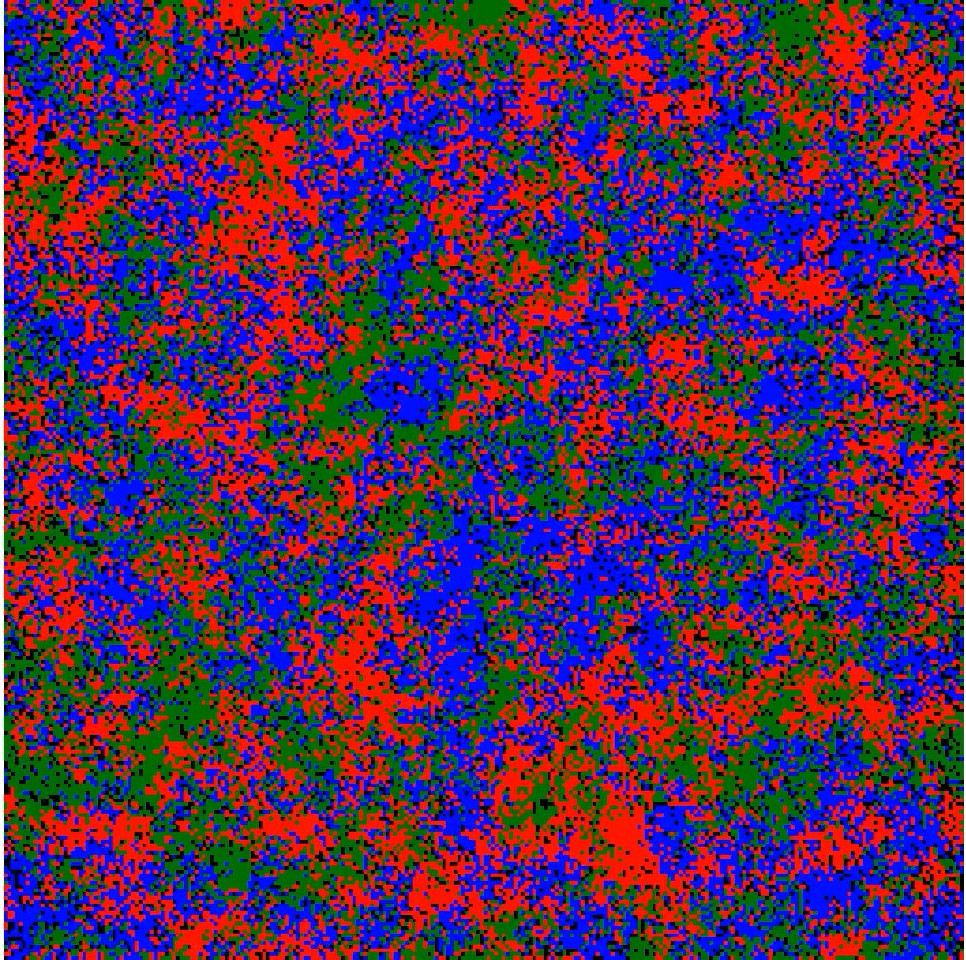
\includegraphics[width=0.24\linewidth]{images/rps_1_25.jpg} }}
            \subfloat[$\epsilon_r=5.0$]{{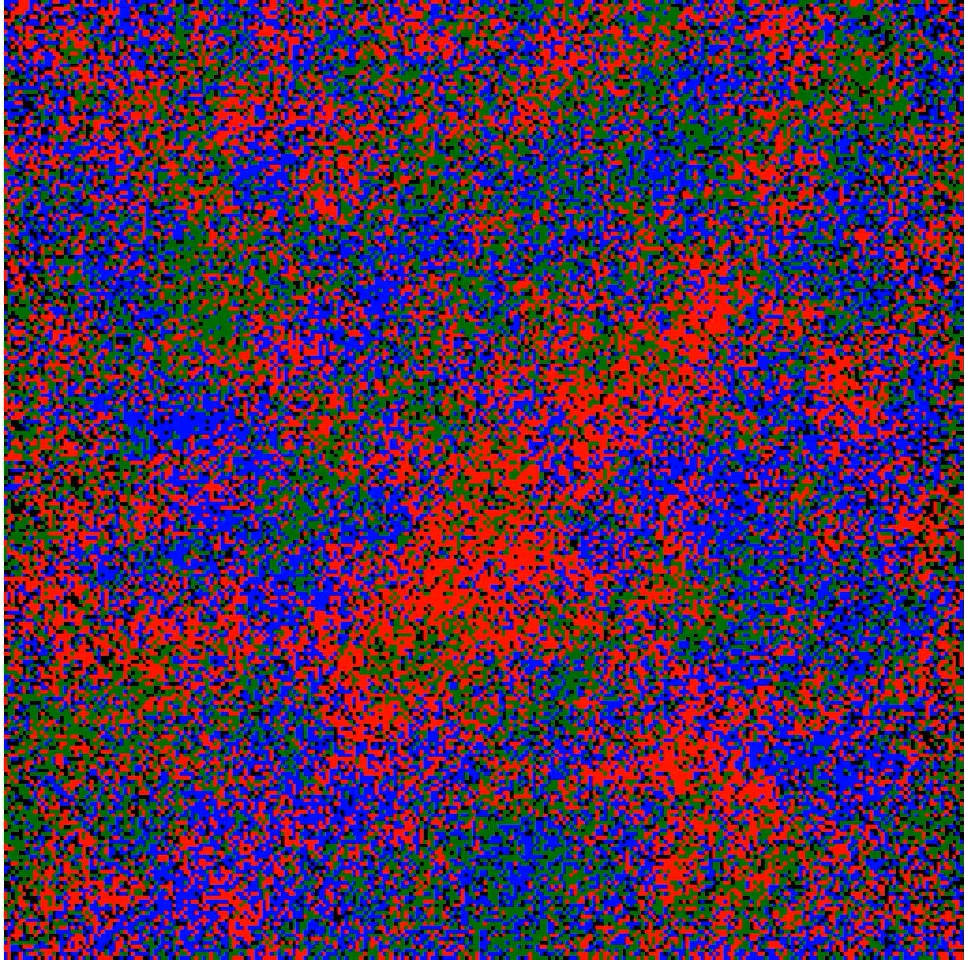
\includegraphics[width=0.24\linewidth]{images/rps_5_0.jpg} }}
            \subfloat[$\epsilon_r=10.0$]{{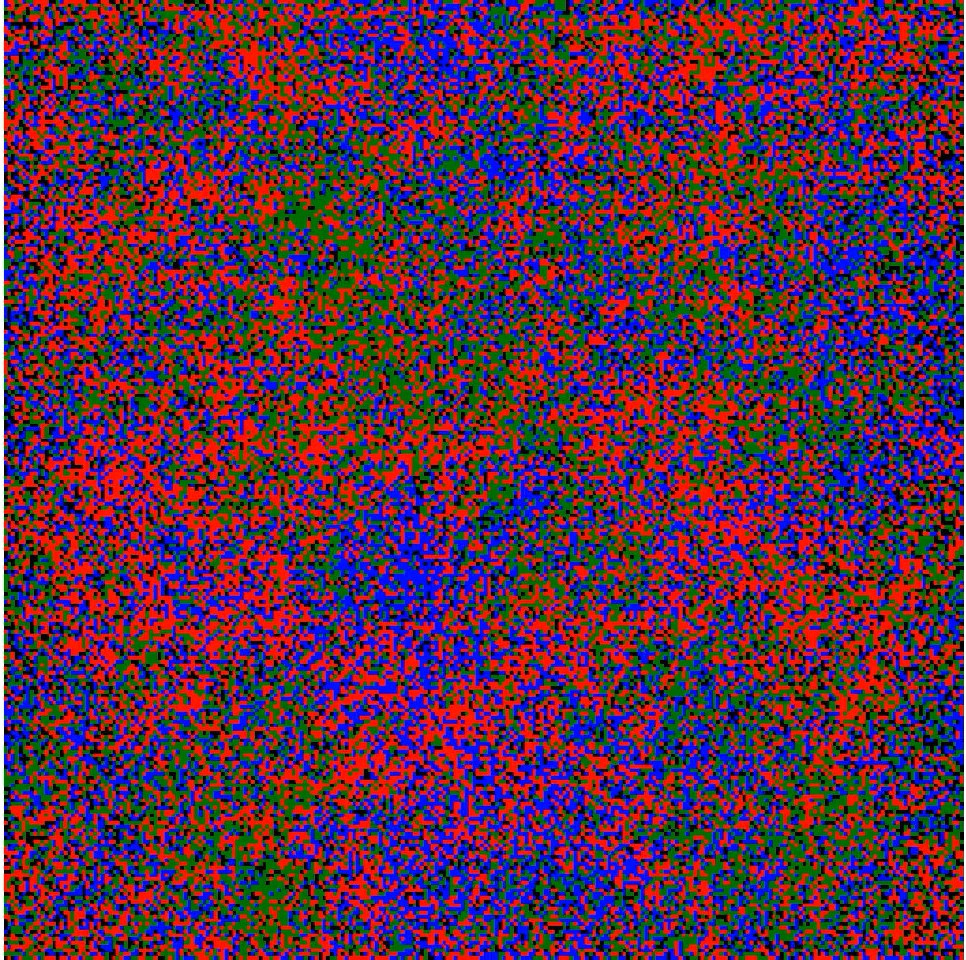
\includegraphics[width=0.24\linewidth]{images/rps_10_0.jpg} }}
            \caption{\centering Steady state snapshots. All lattices have $L_x = L_y = 256$: \\ 
            (a)-(d) Typical ML pattern formation. $\sigma = \sigma = \mu = 1.0$  (e)-(h) Typical RPS pattern formation. $\zeta = 1.0$.}
            \label{fig:patterns}
        \end{figure}
        Our simulations produce (quasi-)stable patterns similar to those seen by Qian He \textit{et al.} \cite{he2011} and Peltom{\"a}ki and Alava \cite{peltomaki08}.

    \end{block}
    \begin{block}{\centering Plane Wave Formation}
        \begin{figure}[h]
            \centering
            \subfloat[$\epsilon_r=0.1$]{{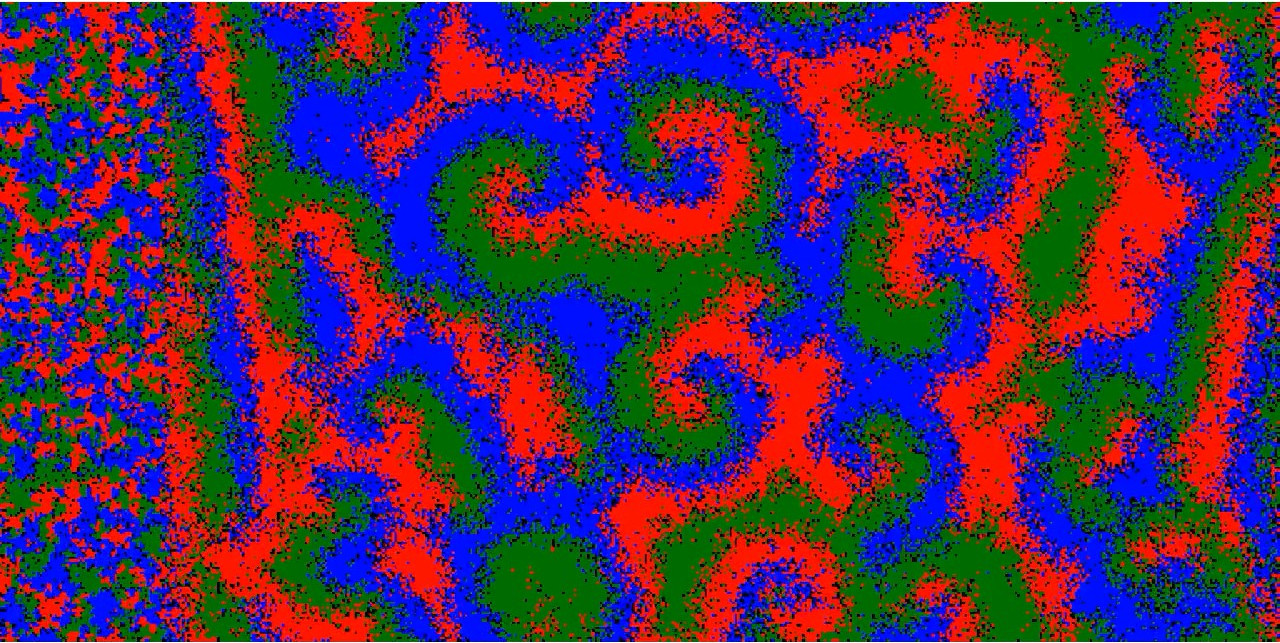
\includegraphics[width=0.48\linewidth]{images/mlrps_0_1.jpg} }}
            \subfloat[$\epsilon_r=2.5$]{{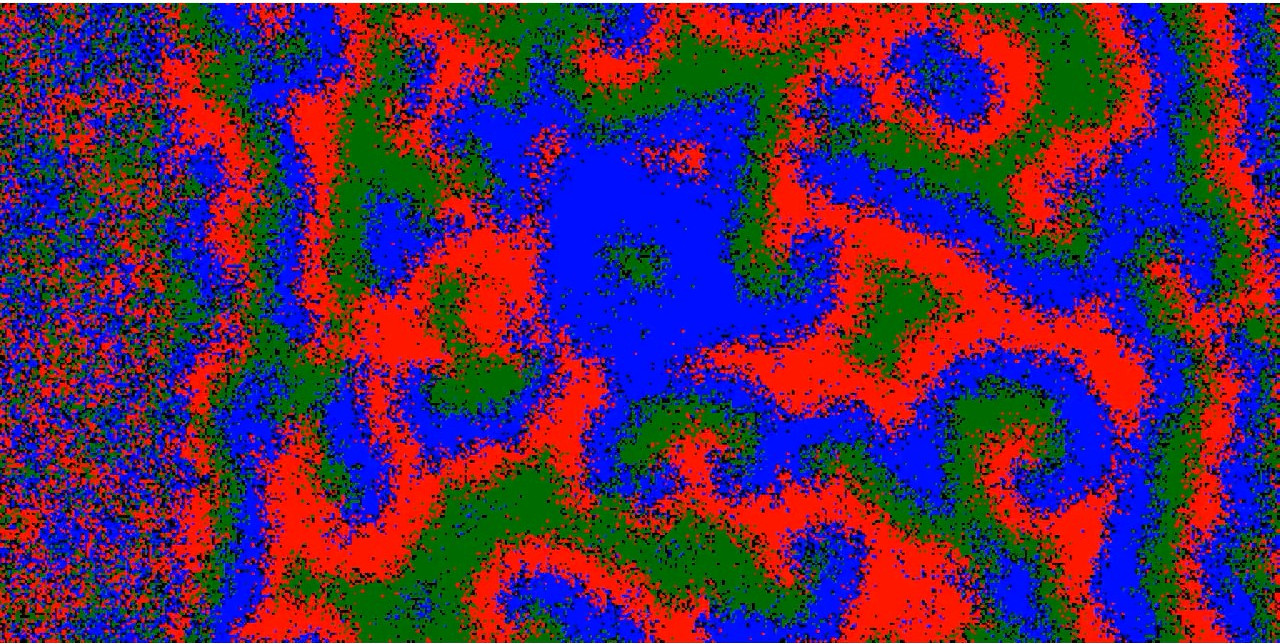
\includegraphics[width=0.48\linewidth]{images/mlrps_2_5.jpg} }}
            \\
            \subfloat[$\epsilon_r=5.0$]{{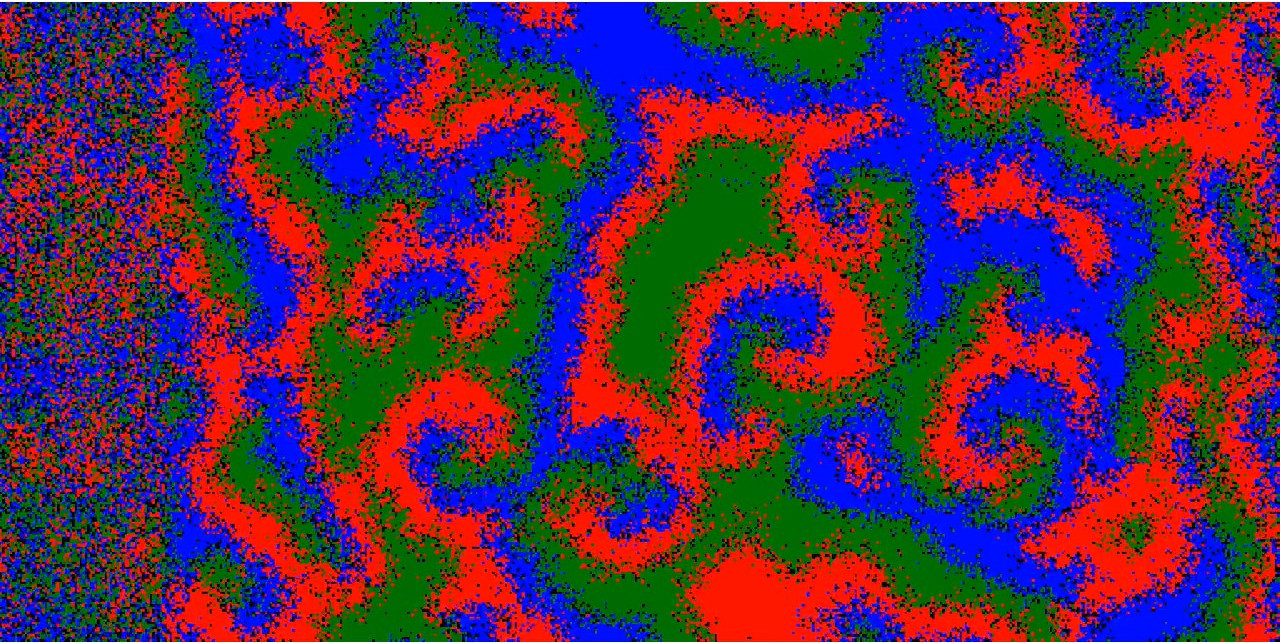
\includegraphics[width=0.48\linewidth]{images/mlrps_5_0.jpg} }}
            \subfloat[$\epsilon_r=10.0$]{{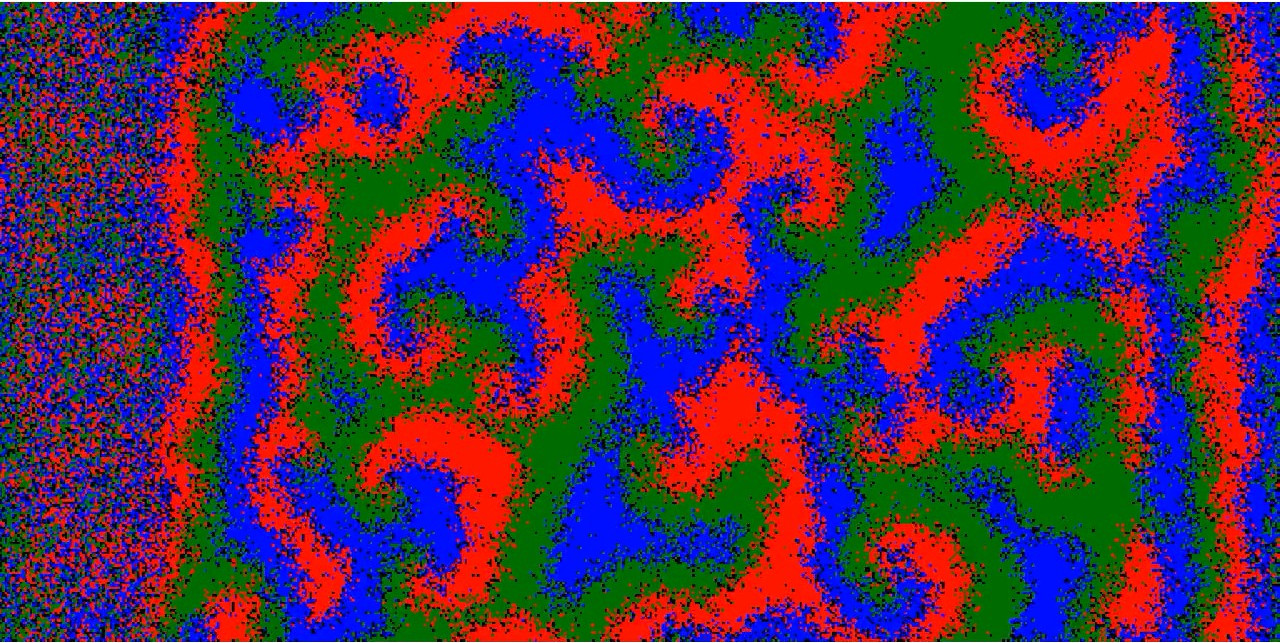
\includegraphics[width=0.48\linewidth]{images/mlrps_10_0.jpg} }}
            \caption{\centering Steady state snapshots of plane wave formation in $256 \times 512$ lattices. In all cases $\epsilon_m = 2.5, \ \sigma = \mu = 1.0, \ \zeta = 1.0$. The interface is placed at $y = 64$.}
            \label{fig:plane_waves}
        \end{figure}
    \end{block}
    \hfill
    \begin{center}
        
\includegraphics[width=0.25\linewidth]{images/vt_logo.jpg}
    \end{center}
    \hfill
\end{textblock}

\begin{textblock}{0.32}(0.67,0.015)
    %\begin{block}{Characteristic Dynamics of the ML Model}
    %The following values were derived analytically by \textit{Reichenbach, et. al.} \cite{reichenbach08} 
    %\begin{align*}
    %\text{Diffusion Constant:} \quad & D = \epsilon_m d^{-1} N^{-2 / d} \\
    %\quad & \text{where } d \text{ is the number of spatial dimensions}\\
    %\quad & \text{and } N \text{ is the size of the lattice.}\\
    %\text{Constants:} \quad & c_1 = \frac{1}{2}\frac{\mu\sigma}{3\mu + \sigma}, \quad  c_3 = \frac{\sqrt{3}\left(18\mu + 11\sigma\right)}{48\mu + 11\sigma}\\
    %\text{Spreading Velocity:} \quad & v^* = 2 \sqrt{c_1 D}\\
    %\text{Wavelength:} \quad & \lambda = \frac{2\pi c_3 \sqrt{D}}{\sqrt{c_1}\left(1 - \sqrt{1 + c_3^2}\right)}\\
%\end{align*}
    %
    %We use these values to contextualize our measurements in the next section.
    %For the cases shown below we use $d=2$ and $N = W \times H = 2^{17},$ 
    %$\sigma = \mu = \zeta = 1.0 , \text{ and } \epsilon_m = 2.5$
        %This yields theoretical values of $D \approx 9.5 \times 10^{-6}$, $ v^* 
        %\approx 0.00218$, and $ \lambda \approx 0.18$
    ~
    \vfill
    \begin{block}{\centering Plane Wave Behavior}
        In Fig. \ref{fig:plane_waves} we see the formation of plane waves at
        the interface between the ML and RPS regions. The plane waves appear to be
        stable features of the interface. Furthermore, initial visual inspection
        seems to indicate that the coherence of these plane-waves seems to be 
        dictated by both $ \epsilon_m $ and $ \epsilon_r $. Further numerical
        analysis is required to confirm this, however.
    \end{block}%\end{block}

    \begin{block}{\centering Well-Mixing Effects}
        \begin{figure}[h]
            \centering
            \subfloat[Net density vs. time for a variety of $ \epsilon_m $ values.
            Here we can clearly see the transient minimum caused by the homogeneous
            initial conditions.]{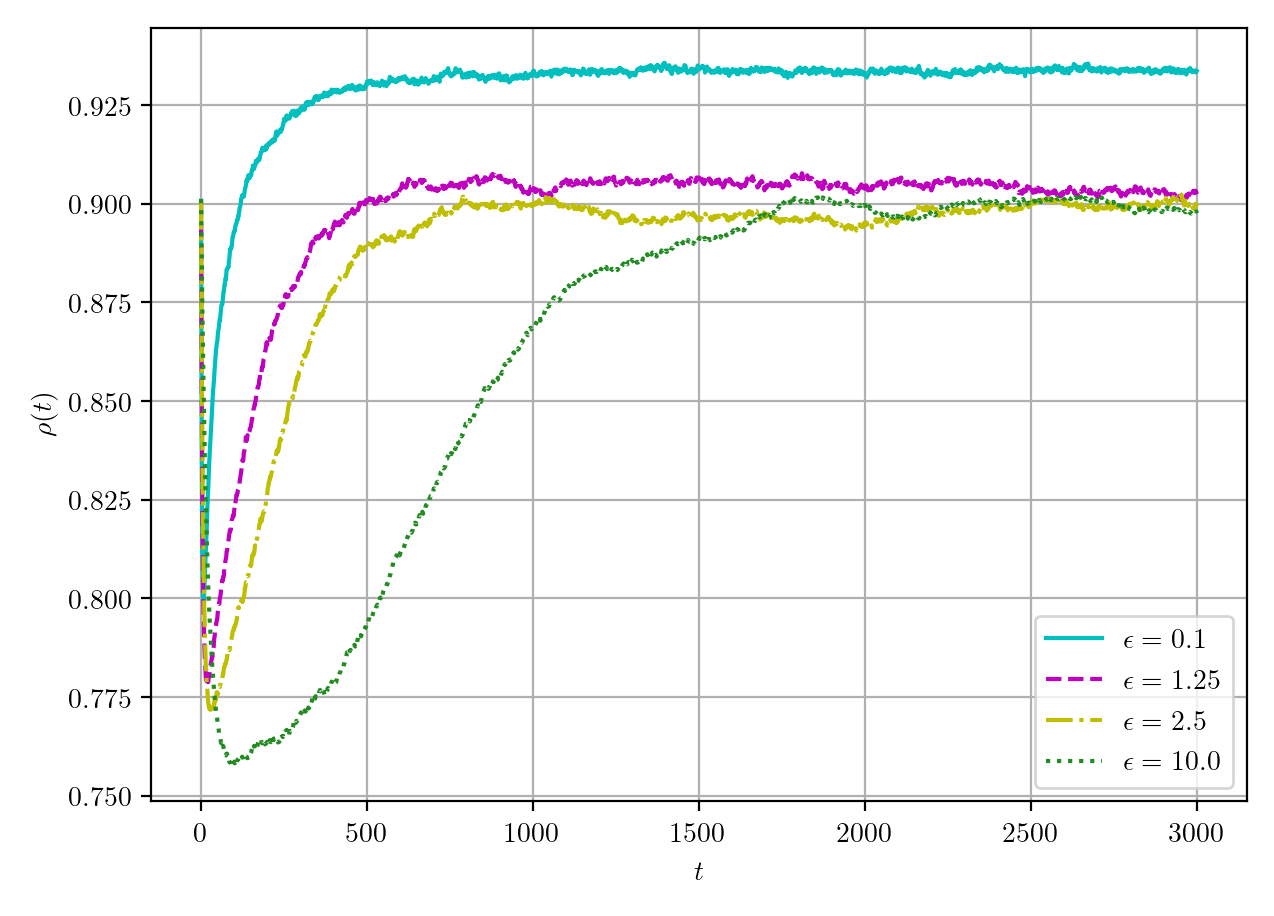
\includegraphics[height = 4.0in]{images/densities_try_0.png}}
            \quad
            \subfloat[Net population density at $ t = 3000 \mathrm{MCS} $ as
            a function of $ \epsilon_m $ ]{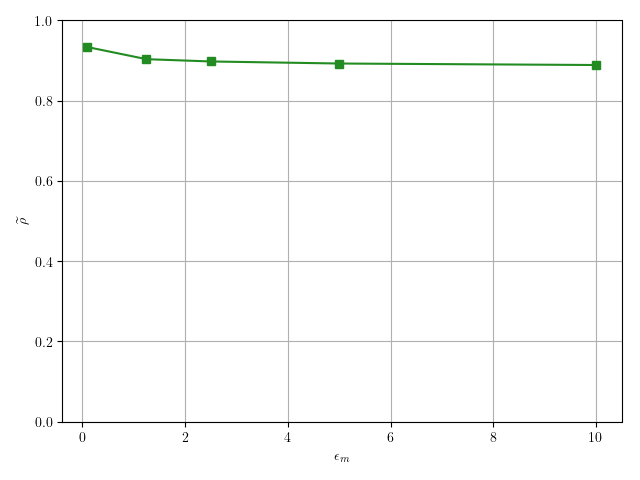
\includegraphics[height = 4.0in]{images/carryingCap2.png}}
            \caption{In the above simulations we set $ \sigma = \mu = 1.0 $ }
            \label{fig:popDens}
        \end{figure}
        We simulate four $ N = 256 \times 256 $ May-Leonard lattices, each with a
        different mobility rate, for 3000 Monte-Carlo steps and track the total 
        population density $ \rho = \frac{n_a + n_b + n_c}{N} $. We begin each 
        simulation from a homogeneous initial condition and an initial density 
        of $ \rho_0 = 0.9 $. In each simulation the total density quickly reaches
        a transient minimum $ \rho_\mathrm{min} $ (Fig. \ref{fig:popDens} (a))
        before relaxing to a steady state density $ \tilde\rho $ determined, in 
        part, by the mobility rate of the system (Fig. \ref{fig:popDens} (b)). Note that in each simulation 
        $ \rho_\mathrm{min} \sim \rho^* = 3 \left( \frac{\mu}{3\mu + 
        \sigma}\right) = 0.75$, where $ \rho^* $ is the mean field steady-state
        density \cite{he2011}.
    \end{block}

    \begin{block}{\centering Interface Density Effects}
        \begin{figure}[h]
            \centering
            \subfloat[$\epsilon_m=0.1$]{{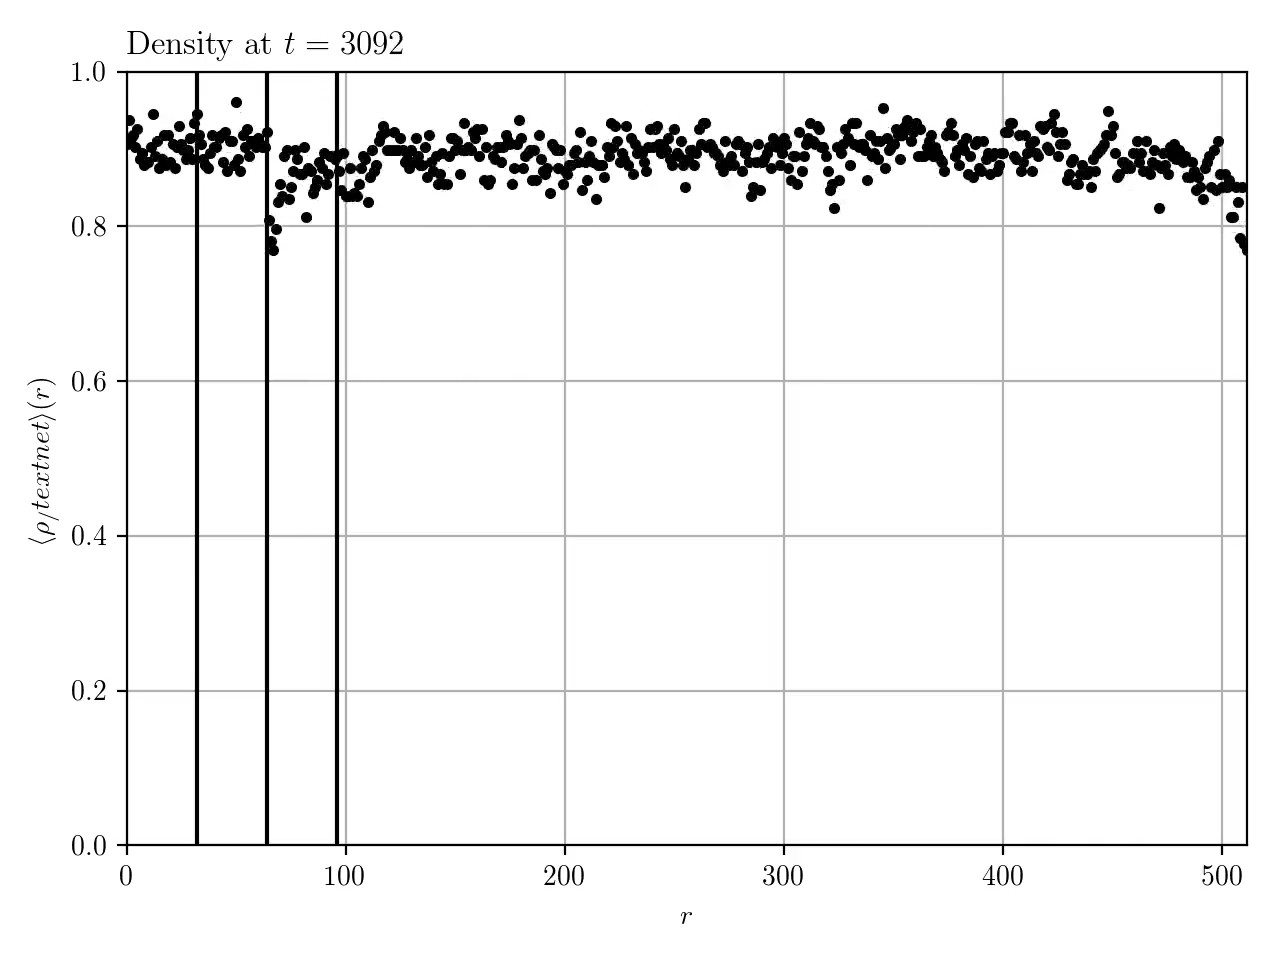
\includegraphics[width=0.3\linewidth]{images/net_density_0_1.jpg}}}
            \subfloat[$\epsilon_m=5.0$]{{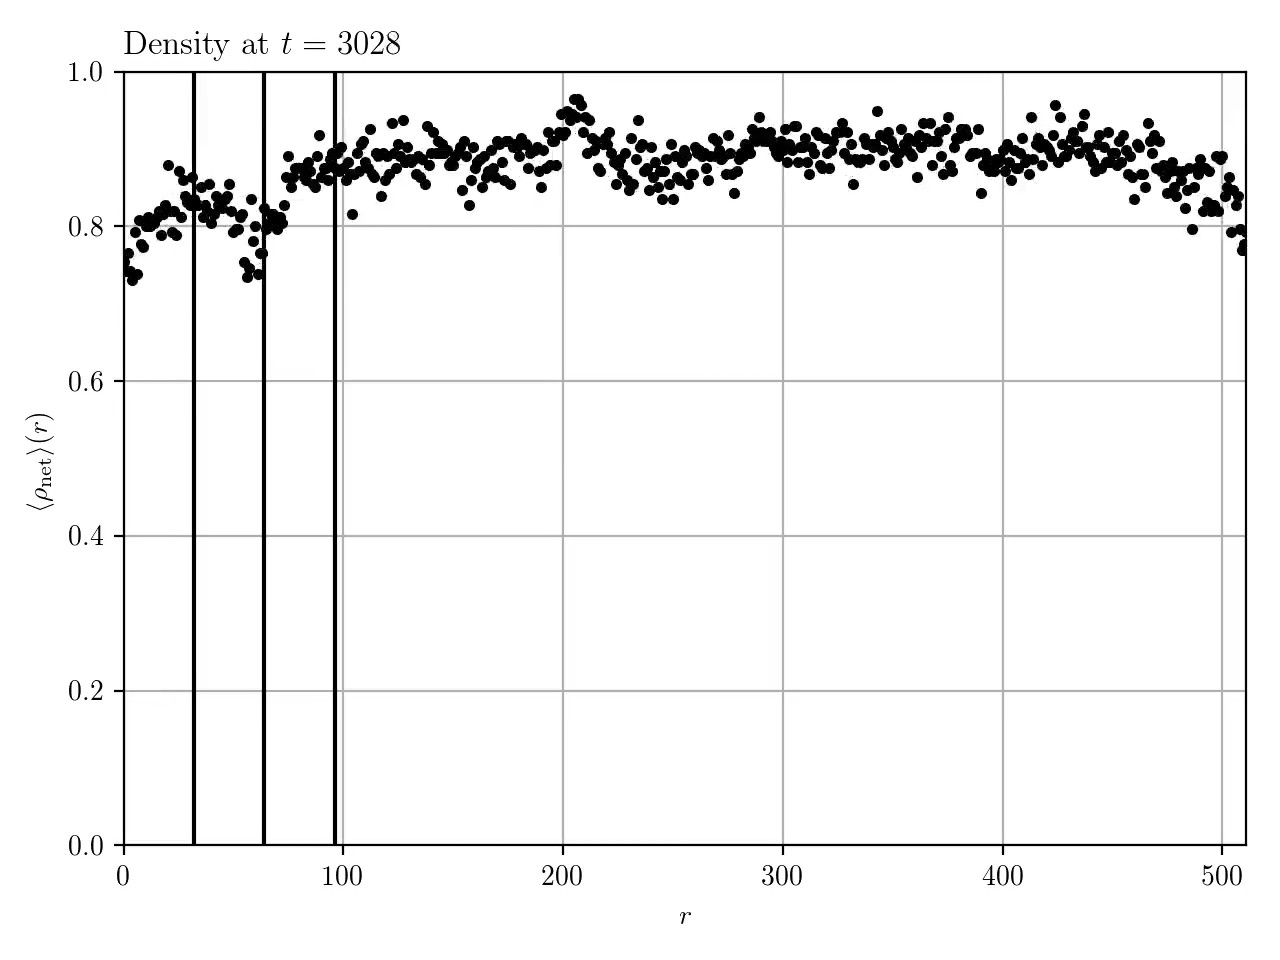
\includegraphics[width=0.3\linewidth]{images/net_density_5_0.jpg}}}
            \subfloat[$\epsilon_m=10.0$]{{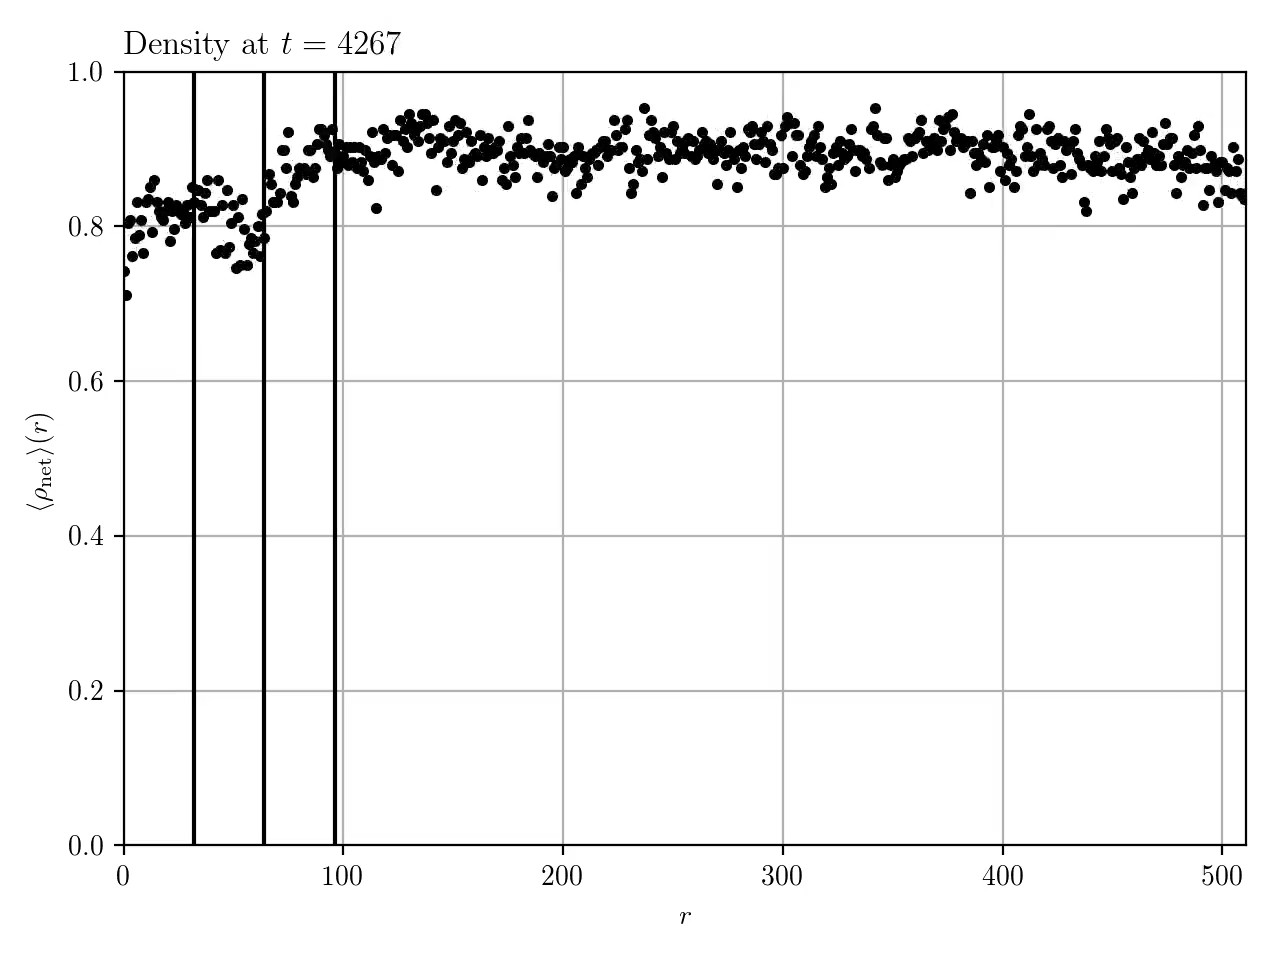
\includegraphics[width=0.3\linewidth]{images/net_density_10_0.jpg}}}
            \caption{\centering Typical interface density effects in $256 \times 512$ lattices for various mobility rates. In all cases $\ \sigma = \mu = 1.0, \ \zeta = 1.0$. The interface is placed at $y = 64$.}
            \label{fig:void}
        \end{figure}
        We observe a marked drop in density near the interface between the RPS and
        ML regions (the center black line in Fig. \ref{fig:void}). This is likely
        caused by a local increase in spatial homogeneity induced by the RPS region. 
        This appears to be similar to the transient minima that we observe above.
    \end{block}

    \begin{block}{\centering Ongoing and Future Work}
        \begin{itemize}
            \item We are currently working to quantify their spatial coherence 
                  and permeation distance of the plane waves.
            \item We will also measure local homogeneity and effective reaction 
                  rates near the interface to confirm that the local mixing
                  is the cause of the drop in density.
            \item As we advance our goal of enhancing and/or disrupting the formation
                  of noise induced patterns we will use the understanding that we
                  have developed of these boundary effects to inform potential
                  new control schemes.
        \end{itemize}
    \end{block}

    \begin{block}{\centering References}
        \bibliographystyle{ieeetr}
        \bibliography{references}
    \end{block}

    \begin{block}{\centering Acknowledgement}
        \begin{figure}[h]
            \centering
            
\includegraphics[width=2in]{images/aro_logo_t.png}
            \label{fig:aro_logo}
        \end{figure}
        \centering
        Research was sponsored by the U.S. Army Research Office and was accomplished 
        under Grant Number W911NF-17-1-0156. 
    \end{block}
    ~
    \vfill

\end{textblock}
\end{frame}
\end{document}
